% !TEX encoding = UTF-8 Unicode
\documentclass[a4paper]{article}

\usepackage{color}
\usepackage{url}
\usepackage[T2A]{fontenc} 	% enable Cyrillic fonts
\usepackage[utf8]{inputenc} % make weird characters work
\usepackage{graphicx}
\usepackage{amsmath}
\usepackage{enumitem}
\usepackage{mathtools}
\usepackage[english,serbian]{babel}
%\usepackage[english,serbianc]{babel}
\usepackage{listings}
\usepackage{wrapfig}
\usepackage{multicol}
\usepackage{epigraph}
\usepackage[unicode]{hyperref}

%%%% Ovi su mozda visak
\usepackage[colorinlistoftodos]{todonotes}
\usepackage{enumitem}
\usepackage{filecontents}
\usepackage{verbatim}
\usepackage{eurosym}
\usepackage[export]{adjustbox}
%%%%

\hypersetup{colorlinks,citecolor=green,filecolor=green,linkcolor=blue,urlcolor=blue}

\graphicspath{ {./images/} }

\newtheorem{primer}{Primer}[section]

\definecolor{mygreen}{rgb}{0,0.6,0}
\definecolor{mygray}{rgb}{0.5,0.5,0.5}
\definecolor{mymauve}{rgb}{0.58,0,0.82}

\lstset{ 
  backgroundcolor=\color{white},
  basicstyle=\scriptsize\ttfamily, % the size of the fonts that are used for the code
  breakatwhitespace=false,         % sets if automatic breaks should only happen at whitespace
  breaklines=true,                 % sets automatic line breaking
  captionpos=b,                    % sets the caption-position to bottom
  commentstyle=\color{mygreen},    % comment style
  deletekeywords={...},            % if you want to delete keywords from the given language
  escapeinside={\%*}{*)},          % if you want to add LaTeX within your code
  extendedchars=true,              % lets you use non-ASCII characters; for 8-bits encodings only, does not work with UTF-8
  firstnumber=1000,                % start line enumeration with line 1000
  frame=single,	                   % adds a frame around the code
  keepspaces=true,                 % keeps spaces in text, useful for keeping indentation of code (possibly needs columns=flexible)
  keywordstyle=\color{blue},       % keyword style
  language=Python,                 % the language of the code
  morekeywords={*,...},            % if you want to add more keywords to the set
  numbers=left,                    % where to put the line-numbers; possible values are (none, left, right)
  numbersep=5pt,                   % how far the line-numbers are from the code
  numberstyle=\tiny\color{mygray}, % the style that is used for the line-numbers
  rulecolor=\color{black},         % if not set, the frame-color may be changed on line-breaks within not-black text (e.g. comments (green here))
  showspaces=false,                % show spaces everywhere adding particular underscores; it overrides 'showstringspaces'
  showstringspaces=false,          % underline spaces within strings only
  showtabs=false,                  % show tabs within strings adding particular underscores
  stepnumber=2,                    % the step between two line-numbers. If it's 1, each line will be numbered
  stringstyle=\color{mymauve},     % string literal style
  tabsize=2,	                   % sets default tabsize to 2 spaces
  title=\lstname                   % show the filename of files included with \lstinputlisting; also try caption instead of title
}

%%%%%%%%%%%%%%%%%%%%%%%%%%%%%%%%%%%%%%%%%%%%%%%%%%%%%%%%%%%%%%%%%%%%%%%%%%%%%%%%%%%%%%%%%

\begin{document}

\begin{titlepage}

\newcommand{\HRule}{\rule{\linewidth}{0.2mm}} 		% change here

\center
 
%----------------------------------------------------------------------------------------
%	HEADING SECTIONS
%----------------------------------------------------------------------------------------

\textmd{\huge Matematički fakultet}\\[0.5cm]
\textmd{\Large Računarska inteligencija}\\[3cm]
%\textsc{\large Assignment 1}\\[0.5cm] % Minor heading such as course title

%----------------------------------------------------------------------------------------
%	TITLE SECTION
%----------------------------------------------------------------------------------------

\HRule \\[0.4cm]
{\huge \bfseries NEAT algoritam za igranje igrice}		\\[0.2cm]
\HRule \\[0.5cm]

{ \Large{NeuroEvolution of Augmenting Topologies}}		\\[3cm]
 
%----------------------------------------------------------------------------------------
%	AUTHOR SECTION
%----------------------------------------------------------------------------------------

\begin{flushleft} \large
\Large{Filip Jovanović 	\hspace{0.75cm} 98/2015		}  	\\
\Large{Stefan Kapunac	\hspace{0.35cm} 157/2015	} 	\\
\Large{Nenad Ajvaz		\hspace{1cm} 316/2015	}	\\[2cm]
\end{flushleft}

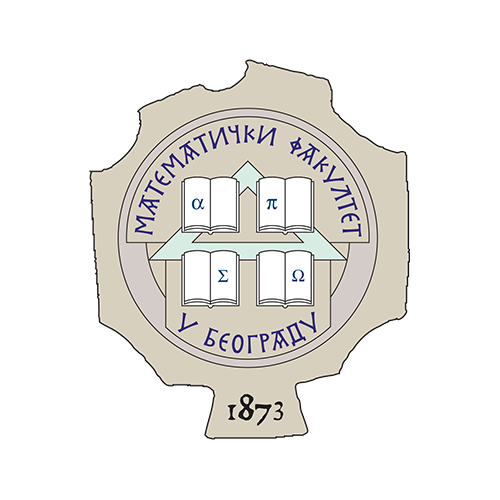
\includegraphics[width=150px, keepaspectratio]{matf.png}\\

{\large{Maj 2019.}}

\vfill % Fill the rest of the page with whitespace

\end{titlepage}

%----------------------------------------------------------------------------------------

\abstract{
U uvodu ćemo ukratko predstaviti NEAT algoritam, a u nastavku se nalazi opis problema koji ovaj projekat treba da reši. U poglavlju \ref{implementacija} će biti predstavljena struktura projekta kao i kratko objašnjenje implementacije, a u poglavlju \ref{podesavanje} prikaz koliku ulogu podešavanje parametara ima u uspešnom radu neuronske mreže.
}

\tableofcontents

\newpage

\section{Uvod}
\label{sec:uvod}

NEAT je tehnika treniranja neuronske mreže genetskim algoritmom. Razvili su ga Kenet Stenli i Risto Mikulainen\footnote{~~Kenneth O. Stanley, Risto Miikkulainen} 2002. godine, na Univerzitetu u Teksasu, SAD \cite{NEAT}. Razlikuje se od ostalih neuronskih mreža po tome što, pored težina može da izmeni i topologiju same mreže. Na početku je topologija minimalna (ulazni čvorovi povezani sa izlaznim), ali će se mutacijom kreirati novi čvorovi, kao i nove grane između njih. Ovo je jedna od ključnih osobina NEAT algoritma, jer nalazi minimalnu neuronsku mrežu koja rešava problem, ali ako to problem zahteva, mreža može postati kompleksna.\\
Testovima je pokazano da NEAT nadmašuje i najbolje mreže fiksne topologije kod zahtevnih zadataka sa pojačanim učenjem (\emph{eng. reinforcment learning}).
\\

Ova tehnika, kao i većina neuronskih mreža, se može koristiti u raznim oblastima. Budući da se NEAT oslanja na neuro-evoluciju, njegovi tvorci smatraju da se algoritam veoma dobro snalazi u neprekidnom i visoko-dimenzionom prostoru stanja. Iz tog razloga, ovaj algoritam je primenjiv i na probleme učenja igranja video igara, što ovaj projekat obuhvata. \\
Pored zvanične dokumentacije za ovaj algoritam, koristili smo se i literaturom o veštačkoj inteligenciji u kreiranju video igara \cite{ai_techs}.


\section{Opis problema}
\label{opis_problema}

U prvom delu poglavlja će biti predstavljena sama igra koju mreža treba da savlada, dok ćemo u drugom delu poglavlja objasniti osnovne koncepte NEAT algoritma i njegovu primenu na igrici.

\subsection{Video igra - MouseRun}
\label{mouserun}

Prvi korak projekta bio je osmisliti adekvatnu video igru, koja bi bila dovoljno interesantna za čoveka, ali i posmatranje kako računar pokušava da je savlada. Kako bismo mogli da lako menjamo bilo koji njen segment u cilju poboljšanja parametara za algoritam, igru smo napravili od nule.
Kontroliše se miš čiji je cilj da pobegne od mačke koja ga juri, a to može da uradi samo ako održava energiju jedući sireve, pritom izbegavajući mišolovke i bare koje ga usporavaju. Prikaz igrice na slici \ref{fig:mouserun_img}.

\begin{figure}[!h]
\begin{center}
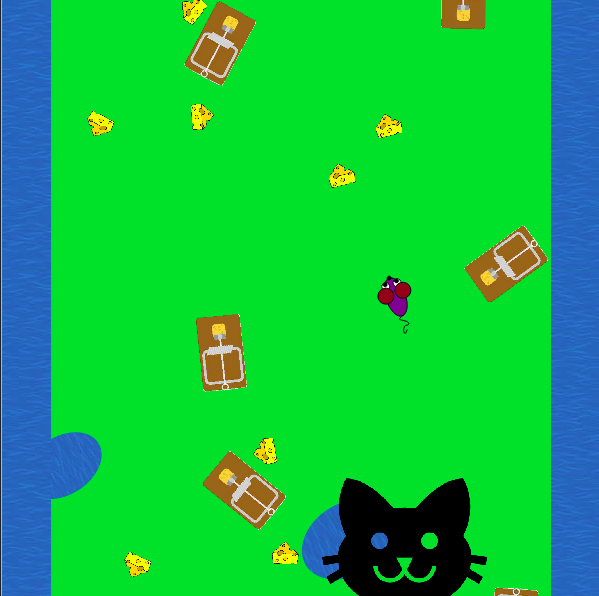
\includegraphics[width=250px, keepaspectratio]{mouse_run_1.png}
\end{center}
\caption{MouseRun}
\label{fig:mouserun_img}
\end{figure}

\subsection{NEAT algoritam}
\label{neat}

Zbog složenije prirode algoritma, neophodan je malo širi uvod, pa će se u nastavku ukratko opisati neki njegovi aspekti, sa osvrtom na neuronske mreže fiksnih topologija i prednosti u odnosu na njih.

\subsubsection*{Neuro-evolucija}
\addcontentsline{toc}{subsection}{\protect\numberline{}2.2.1 ~~Neuro-evolucija}
\label{neuro_evolucija}

Kod tradicionalnih pristupa neuro-evolucije, topologija mreže se bira pre eksperimenta. Obično postoji jedan skriveni sloj čiji su čvorovi povezani sa svim ulazima i izlazima. Prvo se optimizuju težine grana - traže se mreže sa najboljim učinkom, a zatim se one reprodukuju kao čin evolucije, u cilju određivanja funkcionalnosti te mreže. Mana ovakvih fiksnih topologija je što nisu samo težine grana bitne za funkcionalnost, već i struktura, koja je u ovom slučaju nepromenljiva. Takođe, zahteva i ručno određivanje optimalne topologije (broj skrivenih čvorova) za specifičan problem metodom pokušaja i greške.

\subsubsection*{Izazovi u implementaciji}
\addcontentsline{toc}{subsection}{\protect\numberline{}2.2.2 ~~Izazovi u implementaciji}
\label{izazovi}
Prednost NEAT algoritma je u tome što prvo minimizuje strukturu mreže kroz evoluciju, kako bi smanjio dimenzionalnost prostora pretrage težina grana, što dovodi do značajnog ubrzanja kod učenja. Ovo sa sobom nosi nekoliko izazova:

\begin{enumerate}[topsep=1pt, itemsep=-1ex, partopsep=1ex, parsep=1ex]
\item kako odabrati pogodnu genetsku reprezentaciju za ukrštanje
\item kako očuvati topologije kojima je potrebno nekoliko generacija za optimizaciju
\item kako minimizovati topologiju \emph{kroz evoluciju} bez posebnih testiranja kompleksnosti
\end{enumerate}
Rešenja problema su ukratko objašnjena u nastavku. \\

\noindent
\label{reprezentacija}
\textbf{1. Odabir reprezentacije} \\
\indent
Mreže se mogu predstaviti direktnim i indirektnim enkodiranjem. Direktno enkodiranje tačno navodi čvorove i grane u fenotipu\footnote{~~Fenotip je skup osobina organizma koje su nastale zajedničkim delovanjem genotipova i uslova sredine u kojoj se organizam razvija.}, ono je jednostavnije i koriste ga većina mreža.\\
Indirektno kodiranje je kompaktnije - navode se samo pravila za konstruisanje fenotipa, čvorovi i grane se mogu izvesti iz tih pravila. NEAT koristi indirektno kodiranje, jer njihova fleksibilnost može da usmeri pretragu na nepredvidive načine. \\

\noindent
\label{specijacija}
\textbf{2. Očuvanje specijacijom} \\
\indent
Kada se u mrežu doda nova grana, veoma retko će odmah dovesti do poboljšanja performansi. Celokupan fitnes će opasti, jer težina nove grane nije optimizovana. Potrebno je da prođe nekoliko generacija da bi se ta grana poboljšala, ali i u međuvremenu sačuvati da mreža sa takvom nestabilnom strukturom ne bude odbačena.\\
Rešenje toga leži u specijaciji, a ona predstavlja grupisanje organizama u vrste koji imaju slične karakteristike. Kod algoritma NEAT, to se radi preko funkcije \emph{explicit fitness sharing}. Ideja je da se populacija podeli na ,,vrste‘‘ i spreči da neka od vrsti postane dominantna u populaciji, jer ima visok stepen prilagođenosti. To se radi tako što se vrednosti fitnesa normalizuju veličinom trenutne populacije i njihove celokupne sposobnosti. \\

\noindent
\label{specijacija}
\textbf{3. Očuvanje minimalnosti} \\
\indent
Kod određenih vrsta mreža, najlakši način da se očuva minimalnost je smanjivanje fitnesa kad mreža postane velika, ali teško je pogoditi parametar za takvo penalizovanje, jer se mora znati koliko je izračunavanje kompleksno. NEAT ne mora da ima nikakav eksplicitan mehanizam za to, jer uvek kreće od minimalne topologije. Tako je pretraga malih dimenzionalnosti, i raste po potrebi. Ovo se odnosi i na sve usputne međumreže.

\section{Implementacija NEAT algoritma}
\label{implementacija}

U nastavku će ukratko biti opisani najbitniji delovi klasa programa, a zatim princip rada važnijih delova algoritma.

\subsection{Struktura programa}
\label{struktura}

\begin{itemize}

\item \textbf{Genome} - reprezentacija jedne instance neuronske mreže. Sadrži listu čvorova i grana mreže, broj ulaza, izlaza, slojeva i koeficijent fitnesa kao merilo prilagođenosti. Sadrži funkciju koja prolazi kroz mrežu i na osnovu njene uspešnosti daje različite komande miševima. Genom može i da se ukršta i mutira.

\item \textbf{NodeGene} - predstavlja čvor mreže. Svaki čvor pamti identifikator, u kom se sloju nalazi, sa kim je povezan i izlaznu vrednost koju propagira kroz mrežu nakon aktivacije.

\item \textbf{ConnectionGene} - predstavlja granu mreže. Čuva ulazni i izlazni čvor, težinu i inovativni broj\footnote{~~Broj koji predstavlja jedinstvenu globalnu oznaku gena.}.

\item \textbf{Species} - predstavlja vrste unutar generacije. U njoj se nalaze slične instance klase \emph{Genome}, u kojoj se čuva najbolja i prosečna prilagođenost, najbolja jedinka, kao i indikatori da li je vrsta zaostala. Postoje funkcije za utvrđivanje pripadnosti vrsti, kreiranja nove jedinke, ali i uništavanje vrste ako stagnira.

\item \textbf{Game} - predstavlja instancu jedne partije igre. Pošto jedna partija sadrži nekoliko desetina miševa, pored svih njih pamti i identifikator najboljeg.

\item \textbf{Controller} - glavni pokretač celog programa. Sadrži listu genoma kao populaciju, listu vrsti kojoj ti genomi pripadaju kao i broj generacija kroz koje mreža treba da prođe. U ovoj klasi se nalazi najbitnija funkcija \emph{evolve}, koja primenjuje genetskog algoritma na mrežu.

\end{itemize}

\subsection{Bitni koncepti}

\textbf{Mutacija} kod NEAT algoritma ne menja samo težine grana, već i topologiju mreže - tako raste od minimalne ka optimalnoj. Topologija mreže može se izmeniti na dva načina:
\begin{enumerate}[topsep=1pt, itemsep=-1ex, partopsep=1ex, parsep=1ex]
\item \textbf{dodavanje grana} - nova grana se stvara i spaja dva do sad nepovezana čvora, a težina grane se određuje na slučajan način.
\item \textbf{dodavanje čvorova} - postojeća grana se deli i onemogućava, zatim se pravi novi čvor na njoj koji je povezan sa ista dva čvora kao i prethodna grana. Nova grana koja vodi u novi čvor će imati težinu 1, grana koja vodi iz novog čvora će zadržati prethodnu težinu.\\
\end{enumerate}

Kao što je ranije rečeno, dodavanje novih grana ne mora da znači da će postojati negativan uticaj na mrežu, \textbf{specijacijom} se ona može očuvati kroz generacije. Ona funkcioniše tako što za jedinku proveravamo koliko ima sličnu strukturu sa ostalim jedinkama u vrsti, uparimo ih po njihovom inovativnom broju i merimo broj čvorova koji su višak (\emph{eng. excess}) i razdvojeni (\emph{eng. disjoint}). Višak su čvorovi koji se ne podudaraju na kraju, a razdvojeni oni koji se ne podudaraju u sredini. Na slici \ref{fig:genomes} se nalazi primer.

\begin{figure}[!h]
\begin{center}
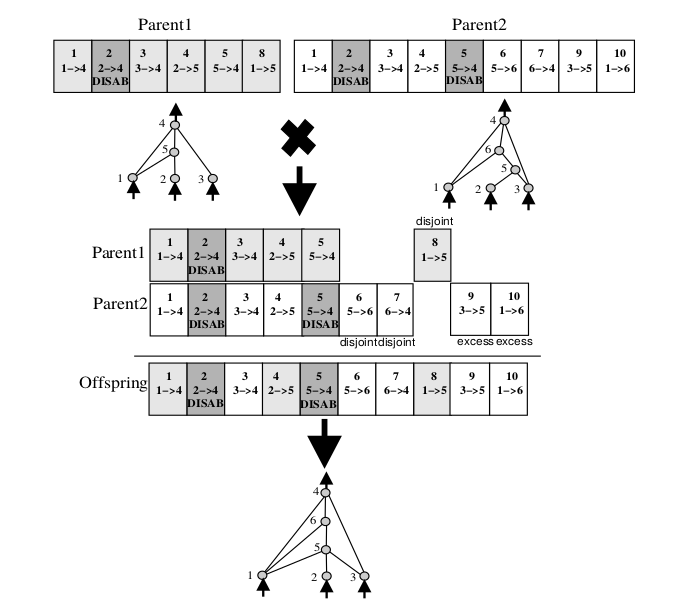
\includegraphics[width=190px, keepaspectratio]{matching.png}
\end{center}
\caption{Poklapanje čvorova dve mreže}
\label{fig:genomes}
\end{figure}

Nakon računanja takvih čvorova, po sledećoj formuli se određuje da li će jedinka pripasti vrsti:

\begin{center}
$\delta = \dfrac{c1 \cdot{E}}{N} + \dfrac{c2 \cdot{D} }{N} + c3 \cdot \overline{W} $, \\
\end{center}
gde je $\delta$ rastojanje podudarnosti, $E$ broj višak čvorova, $D$ broj razdvojenih čvorova, $\overline{W}$ prosečno rastojanje težina kod čvorova koji se podudaraju, a $N$ broj grana u većoj jedinci. Koeficijenti $c1, c2, c3$ su parametri koji balansiraju važnost ova tri faktora. Ako je $\delta$ veće od unapred postavljenog praga $\delta_t$, jedinka pripada vrsti.\\
Ranije smo naveli funkciju \emph{explicit fitness sharing} i njenu ulogu, a sada navodimo kako se ta nova prilagođenost računa za svaki organizam $i$:

\begin{center}
$ f_i' = \dfrac{f_i}{ \sum_{j=1}^{n} sh(\delta(i,j)) } $, \\
\end{center}
gde je $sh(\delta(i,j))=1$ ako je $\delta > \delta_t$, inače je 0.\\

Kada je u pitanju \textbf{ukrštanje} genoma, sličan je postupak kao kod merenja pripadnosti neke jedinke vrsti. Za dve jedinke koje želimo da ukrstimo se prvo poređaju grane sa istim inovativnim brojem, i one se nasumično prosleđuju u dete, dok se geni koji se ne poklapaju nasleđuju od prilagođenijeg roditelja.

\section{Podešavanje parametara i rezultati}
\label{podesavanje}

Veći problem od same implementacije algoritma bio je izbor odgovarajućih parametara - veličina populacije, funkcija cilja kao i ulazne vrednosti za neuronsku mrežu. 

\begin{itemize}

\item \textbf{Veličina populacije} - Zbog hardverskih ograničenja, velike populacije su pravile dva problema:
\begin{enumerate}
\item Ocenjivanje je bilo sporo - ovaj problem smo rešili podelom populacije na manje grupe od 100 jedinki, pa bi se ocenjivanje vršilo po grupama umesto na celoj populaciji odjednom.
\item Stvaranje sledeće generacije je bilo sporo - ovaj problem smo mogli da izbegnemo jedino ograničavanjem veličine populacije na 1000-2000.
\end{enumerate}


\item \textbf{Funkcija cilja} - Početna ideja je bila da ocena za igrača bude vreme koje je uspeo da ostane u životu. Međutim, nastao je problem u tome što se u prvim generacijama najčešće više isplatilo da samo idu napred. Posle mnogo eksperimentisanja, odlučili smo da uvedemo bonuse za svako kretanje, skretanje, izbgavanje prepreka i konzumiranje sira, kao i penale za prolaske kroz bare, stajanje u mestu i kretanje isključivo u jednom smeru.

\item \textbf{Ulazne vrednosti} - Prva zamisao je bila da svaki igrač može da vidi svoju poziciju, rotaciju, kao i poziciju svih ostalih predmeta na sceni. Glavna mana ovog pristupa je bila to što za veliki broj ulaznih vrednosti, evolucija predugo traje. Da bismo redukovali broj ulaznih vrednosti, dali smo igračima tri senzora - jedan ispred njega i po jedan sa svake strane. Senzor govori igraču da li, i koji objekat se nalazi u njegovoj blizini, kao i tačne koordinate objekta. Na ovaj način, broj ulaznih vrednosti za svaki od senzora je 3, što sa pozicijom i rotacijom igrača čini 12 ulaznih vrednosti. Ovo se pokazalo kao optimalno.

\end{itemize}

Sa ovakvom konfiguracijom, nakon celog dana evolucije i nekoliko stotina generacija, miševi su počeli da uspešno izbegavaju neke prepreke, a neki su uspeli i da opstanu iznenađujuće dugo. Neuronske mreže najboljih jedinki su u tom trenutku imale 20-30 neurona raspoređenih u 3-5 slojeva i 20-30 sinapsi. \\

Zbog vremenskih i hardverskih ograničenja, naš cilj da istreniramo savršenog igrača nije ostvaren, ali evolucija i napredak se jasno mogu videti. Čovek je i dalje u staju da postigne bolji rezultat, ali imajući u vidu da je broj neurona i sinapsi čoveka daleko veći od 30, to nije iznenađujuće.


Na slikama ispod se mogu videti stanja igre u početnim fazama.

\begin{figure}[!h]
  \centering
  \begin{minipage}[b]{0.4\textwidth}
    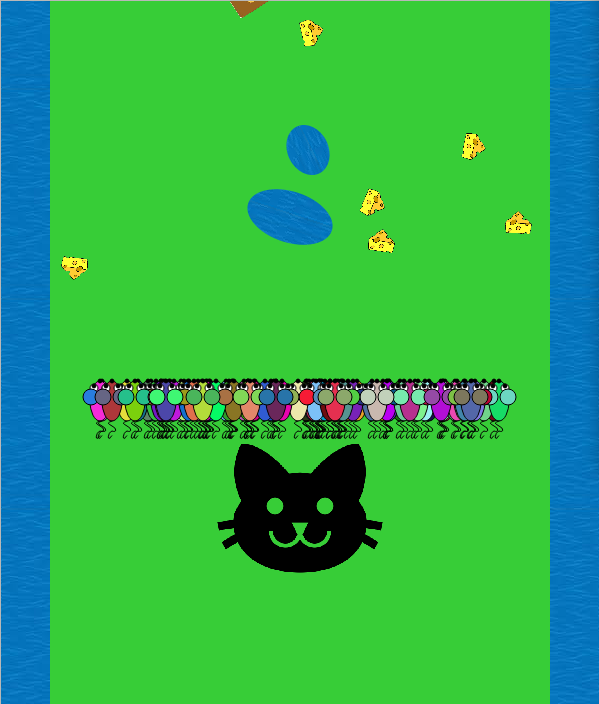
\includegraphics[width=175px]{gen0_batch1.png}
    \caption{Generacija 0, serija 1.}
    \label{fig:gen0batch1}
  \end{minipage}
  \hfill
  \begin{minipage}[b]{0.4\textwidth}
    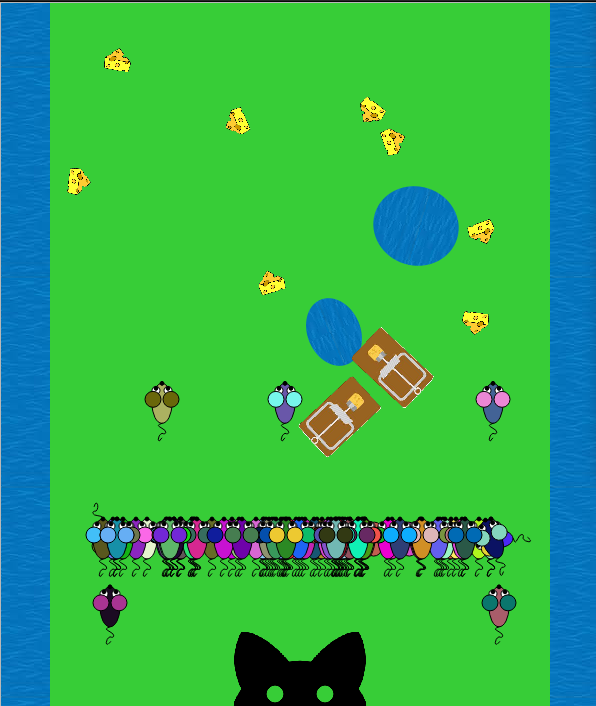
\includegraphics[width=175px]{gen1_batch1.png}
    \caption{Generacija 1, serija 1.}
    \label{fig:gen1batch1}
  \end{minipage}
\end{figure}

\begin{figure}[!h]
  \centering
  \begin{minipage}[b]{0.4\textwidth}
    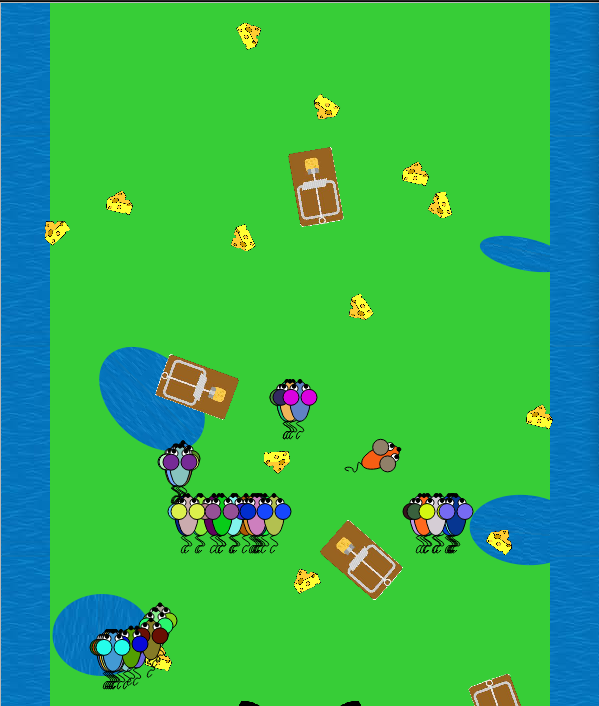
\includegraphics[width=175px]{gen1_batch5.png}
    \caption{Generacija 1, serija 5.}
    \label{fig:gen0batch1}
  \end{minipage}
  \hfill
  \begin{minipage}[b]{0.4\textwidth}
    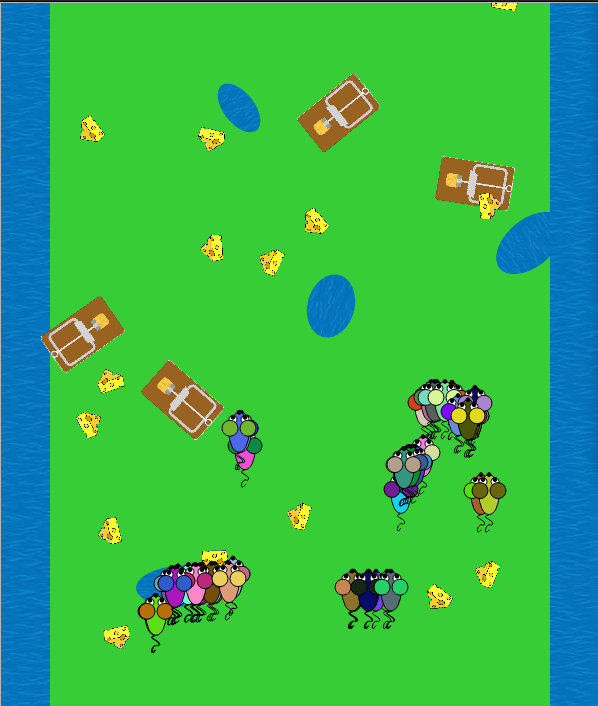
\includegraphics[width=175px]{gen2_batch3.png}
    \caption{Generacija 2, serija 3.}
    \label{fig:gen1batch1}
  \end{minipage}
\end{figure}

\pagebreak

\section{Zaključak}
\label{sec:zakljucak}

NEAT je jedan veoma koristan, ali i dosta kompleksan algoritam. Rezultati koje on daje su vidno bolji od mnogih drugih algoritama sa neuronskim mrežama. Smatramo da je mreža prilično dobro savladala igricu, budući da su najuspešniji pojedinci uspeli da nadmaše najbolji rezultat svakog od autora ovog projekta, iako nismo imali hardver ogromnih performansi za učenje mreže. Danas je ova oblast veoma popularna, i sigurno je da će oblast neuro-evolucije nastaviti da se koristi u problemima raznih sfera.

\pagebreak

\addcontentsline{toc}{section}{Literatura}
\appendix
\bibliography{source} 
\bibliographystyle{ieeetr}

\end{document}